\documentclass[a4paper]{article}
\usepackage{amsmath}
\usepackage{graphicx}
\usepackage{geometry}

\usepackage{layout}
\usepackage{amssymb} 
\usepackage{multirow}
\usepackage{multicol}
\usepackage[font=small,labelfont=bf]{caption}
\usepackage[justification=centering]{caption}
\usepackage{subcaption}
\usepackage[export]{adjustbox}
%\usepackage{subfig}
\usepackage{floatrow}   
\usepackage{listings}
\usepackage{fancyhdr}
\usepackage{xcolor}
\usepackage{cleveref}
\definecolor{codegreen}{rgb}{0,0.6,0} \definecolor{codegray}{rgb}{0.5,0.5,0.5} \definecolor{codepurple}{rgb}{0.58,0,0.82} \definecolor{backcolour}{rgb}{0.95,0.95,0.92} 
\lstdefinestyle{mystyle}{backgroundcolor=\color{backcolour}, commentstyle=\color{codegreen}, keywordstyle=\color{magenta}, numberstyle=\tiny\color{codegray}, stringstyle=\color{codepurple}, basicstyle=\ttfamily\footnotesize, breakatwhitespace=false, breaklines=true, captionpos=b, keepspaces=true, numbers=left, numbersep=5pt, showspaces=false, showstringspaces=false, showtabs=false, tabsize=2 } \lstset{style=mystyle}
\usepackage{siunitx}
\usepackage{titling}
%\geometry{margin=1in}
\usepackage{authblk}
\usepackage{indentfirst}
\usepackage[framemethod=tikz]{mdframed}
\setlength{\droptitle}{-5em}

\newcommand{\fakeimage}{{\fboxsep=-\fboxrule\fbox{\rule{0pt}{3cm}\hspace{4cm}}}}
\def\code#1{\texttt{#1}}

\graphicspath{./C:/vn123/OneDrive/Master/IN5270/Projects/wave_project}

\begin{document}
	\title{\textbf{\huge{Analysis of Bias-Variance Tradeoff}\\ \large{Additional exercise for Project 3}}}
	
	\author{\textbf\large{Sigurd Rustad, Vetle Vikenes, Vetle Nevland}}
	
	\date{\today}
	
	
	\maketitle
	
	
	\section{Introduction}
	The goal of this exercise is to analyse the bias-variance tradeoff using three different machine learning methods. This will provide valuable information of the potential of different methods to solve a particular problem, as well as generalizing to other problems. The training process is at the core of machine learning, ultimately determining how applicable the method is for a set of problems. During training, we want the algorithm to pick up on important features of the data in order to replicate the structure of the data. However, training for too long causes the algorithm to be too tailored at solving the particular problem it has been trained at, and generalizes poorly to other, but similar, kinds of data. To mitigate the loss of generalization, training should stop when the error starts increasing for the test set. The resulting model gives a fair balance between biasedness and overfitting.
	
	\section{Support Vector Machines}
	A machine learning method to be used in this exercise is Support Vector Machines. This method has not been covered in the previous project, so we will provide a brief description of its functionality. \\
	
	Support vector machines is first and foremost a classification method, but can be generalized to regression problems. The idea is to expand a linear decision boundary with a margin $M$ to improve prediction on non-separable classes and nonlinear functions. A general linear regression model is on the form
	\[ f(x) = \beta_0 + x^T\beta \]
	For linear regression the goal is to find the parameters $\beta$ that minimize the squared difference between the model prediction and the target values. For support vector machines the minimization strategy is more extensive. The appropriate cost function penalizes wrong predictions, but ignores the ones with a small residual. This greatly reduces the number of computations needed by the model. We have the following error measure
	\[ V_{\epsilon}(r) = \begin{cases}
		0 & |r| < \epsilon \\
		|r| - \epsilon & \text{else}
	\end{cases} \]
	
	where $r = y - f(x)$ is the prediction error and $\epsilon$ is a constant definining the residual threshold of where to ignore the error. The cost function to minimize involves the error measure $V$ and a penalization term
	
	\[ H(\beta) = \sum_{i=1}^N V_{\epsilon}(r_i) + \frac{\lambda}{2} ||\beta||^2 \]
	Support vector machines is a constrained optimization method, since we want to minimize the squared deviation between the predictions and targets \textit{subject} to a prescribed margin $M$ in the hyperplane. By introducing slack parameters $\xi$ and $\xi^*$ we allow for errors within the margin. Minimizing the loss with respect to all relevant parameters, we get a constrained optimization problem to be solved for relevant parameters, including $\xi$, $\xi^*$, $w$ and $b$. A mathematical derivation is given in \cite{Hastie2009}.
	
	
	
	\section{Data and Methods}
	To avoid the extensive work of implementing a support vector machine from scratch, we resort to Support Vector Regressor (\code{SVR}) provided by scikit-learn. To be consistent, and rather focus on bias-variance analysis, all three methods are adapted from scikit-learn's library.
	
	In the two previous projects we have studied the FrankeFunction in details. We have compared how linear regression and neural network manage to fit a noisy version of the function. The mean squared error have been compared, but not how it's decomposed into bias and variance. The mean squared error can be decomposed as follows.
	
	\[ E\big[(y - \tilde{y})^2\big] = \frac{1}{n}\sum_i (f_i - E[\tilde{y}])^2 + \frac{1}{n}\sum_i (\tilde{y_i} - E[\tilde{y}])^2 + \epsilon \]
	
	The first term represents the bias - the squared sum of individual target points to the expected prediction. The second term represents variance - the squared distance between the expected prediction and each predicted value. The last term is the irreducible error of the model, which will be ignored in this analysis.
	
	The analysis of the mean squared error is extended to include bias-variance tradeoff between linear regression, neural network and support vector machines. The noise used for the FrankeFunction is randomly samples from a standard normal distribution, scaled by a factor $0.2$. \\
	
	The model complexity is a strong indicator of relation between generalization and overfitting, more precisely the decomposition of MSE into bias and variance. The complexity of different methods are represented differently, though, making it necessary to make a clear parametrization of the complexity for the three methods. 
	
	For linear regression we include additional polynomial features. The degree of the polynomial then becomes a new parameter of our model that adjusts the complexity. In addition, using Ridge and Lasso we have an extra regularization parameter $\alpha$ with purpose of reducing large fluctuations caused by a high-dimensional feature space.
	
	For a neural network, model complexity is a function of the architecture of the network. This includes the number of hidden layers, number of hidden nodes, weight initialization and gradient descent method used for updating. The model complexity thus has a more complex parametrization than for linear regression. To avoid making the analysis too comprehensive, we restrict ourselves to the number of hidden layers and number of hidden nodes (using the same number of nodes per hidden layer).

	For support vector machines the model complexity is determined by how large we want the minimum margin to be and how small we want the net residual to be. For \code{SVR} from scikit-learn, this is controlled by the parameter $C$, which act as a regularization term. A low $C$ corresponds to a large span of margin. This implies that more points fall within the margin and are penalized, hence a lower model complexity. On the contrary, a large $C$ gives minor regularization and will make the net residual closer to zero. This is achieved by a high model complexity. Epsilon is another parameter of SVM, determining how large we allow residuals to be for them to be ignored (not included in the minimization). We will focus on the $C$ parameter and set a prescribed $\epsilon = 0.2$. The chosen kernel - the custom subspace to perform predictions in - will affect the performance of \code{SVR}. FrankeFunction including noise is highly nonlinear, thus we choose a radial basis function kernel rather than a linear kernel.
	
	
	
	\section{Results and Discussion}
	All results presented in this exercise are obtained by the python programs located in the folder \code{code\_extra} and are reproducible. Running the \code{main.py} file will produce the most important results used in the bias-variance analysis. All errors presented are result of bootstrap simulation of the algorithms.
	
	\subsubsection*{Linear Regression}
	
	\begin{figure}[h]
		
		\centering
		\begin{subfigure}{0.49\textwidth}
			\centering
			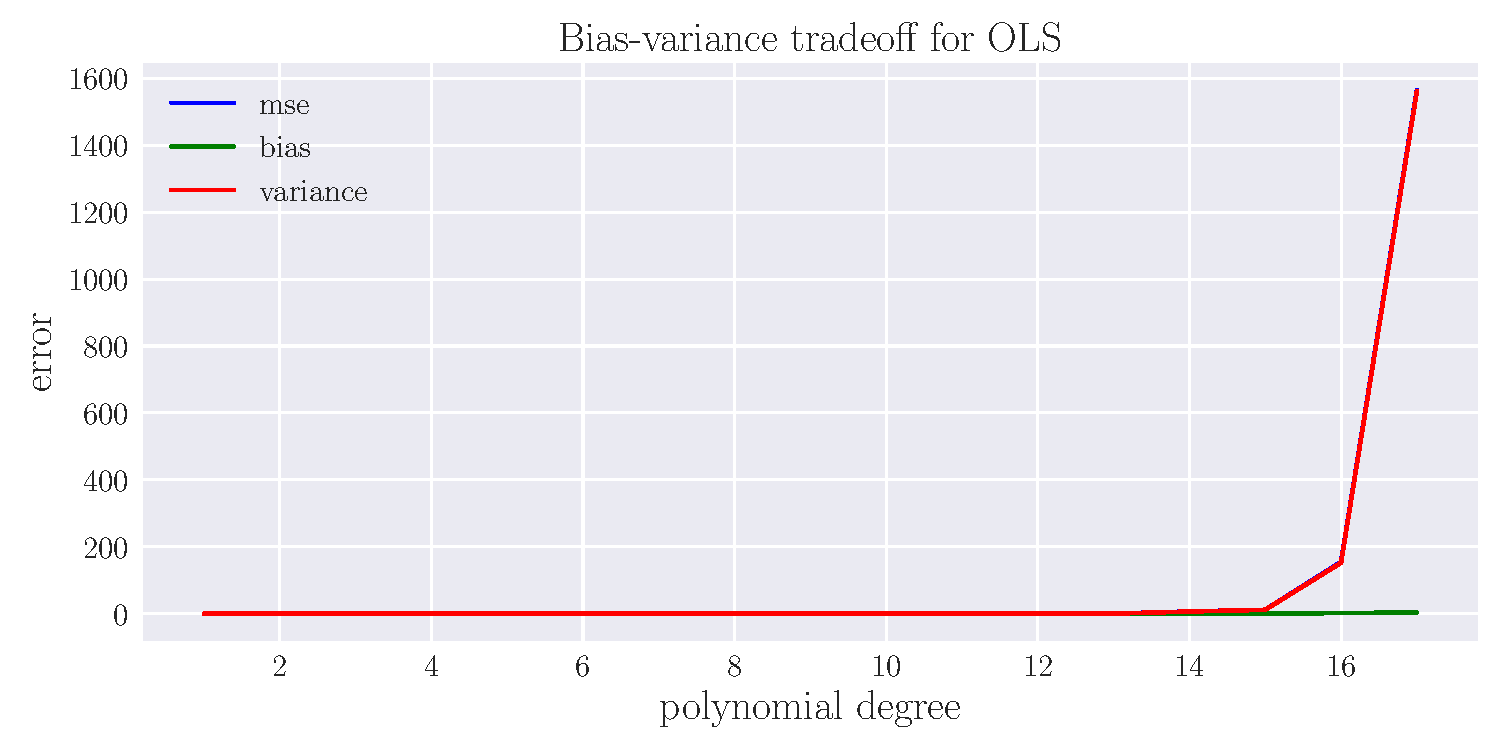
\includegraphics[width=\textwidth]{../output_extra/plots/bias_var_OLS_c17.pdf}
			\caption{Max degree 17}
			\label{fig:OLS_a}
		\end{subfigure}
		\hfill
		\begin{subfigure}{0.49\textwidth}
			\centering
			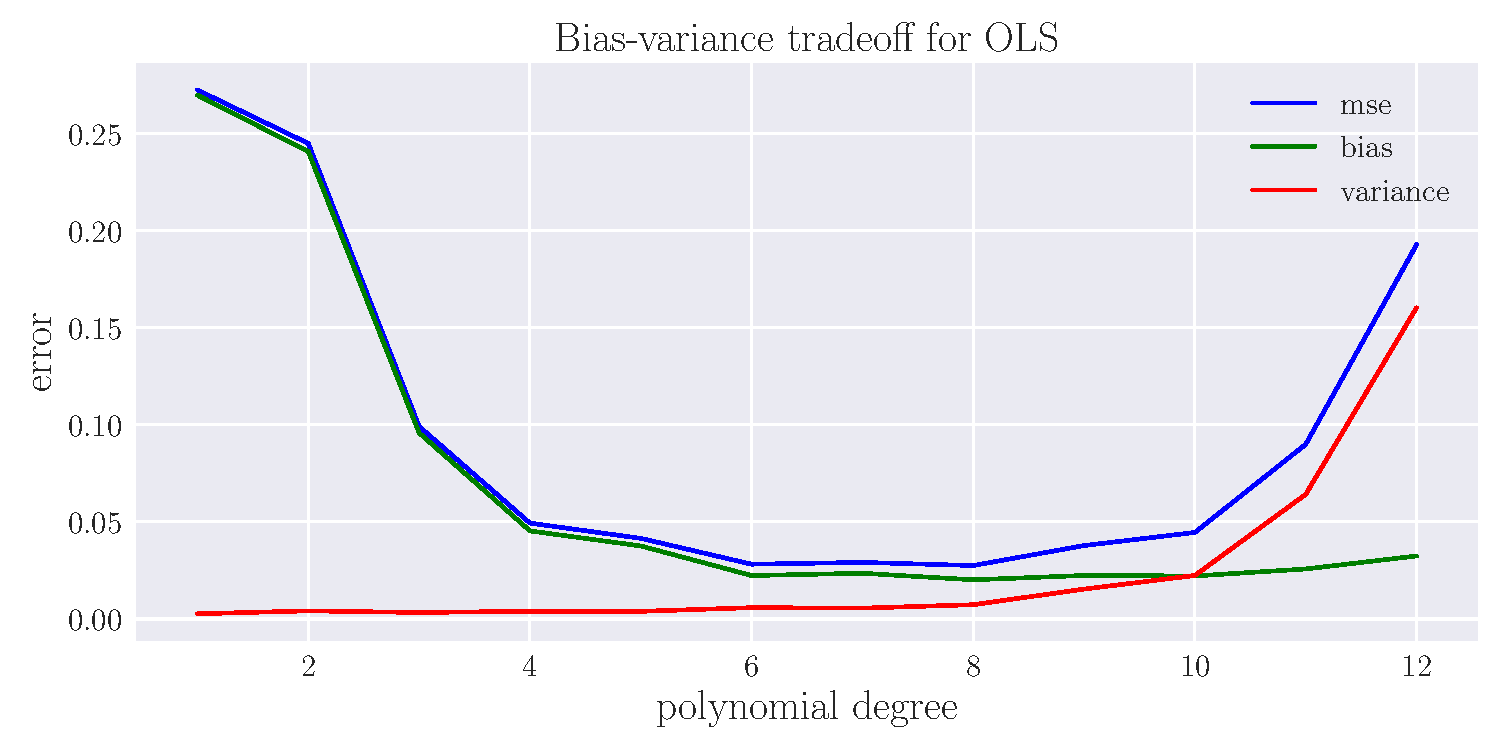
\includegraphics[width=\textwidth]{../output_extra/plots/bias_var_OLS_c12.pdf}
			\caption{Max degree 12}
			\label{fig:OLS_b}
		\end{subfigure}
		\caption{Bias-variance tradeoff as a function of polynomial degrees for OLS, simulated on FrankeFunction.}
		\label{fig:OLS}
	\end{figure}
	
	The results from running linear regression on FrankeFunction are essentially the same as those obtained in project 1. Figure \ref{fig:OLS} shows the MSE and the decomposition into bias and variance. The left plot, Figure \ref{fig:OLS_a}, illustrates for polynomial degree up to order 17. Overfitting clearly dominates for polynomial degrees around 15 and higher. The MSE explodes for this model complexity, making it hard to analyse for lower order complexities as they are deafed by the exploding MSE. 
	The right plot, \ref{fig:OLS_b}, shows the bias-variance tradeoff up to order 12. This better illustrates the development of MSE as model complexity increases. A minimum MSE seems to be reached for a polynomial degree between 6 and 8. The bias decreases significantly less for low polynomial degrees than the variance increases for high polynomial degrees, as clearly illustrated in Figure \ref{fig:OLS_b}. Hence, overfitting is certainly a more severe problem than underfitting. This is as expected, as OLS will suffer from highly fluctuating regression parameters as the complexity gets high. \\
	
	\begin{figure}[h]
		
		\centering
		\begin{subfigure}{0.49\textwidth}
			\centering
			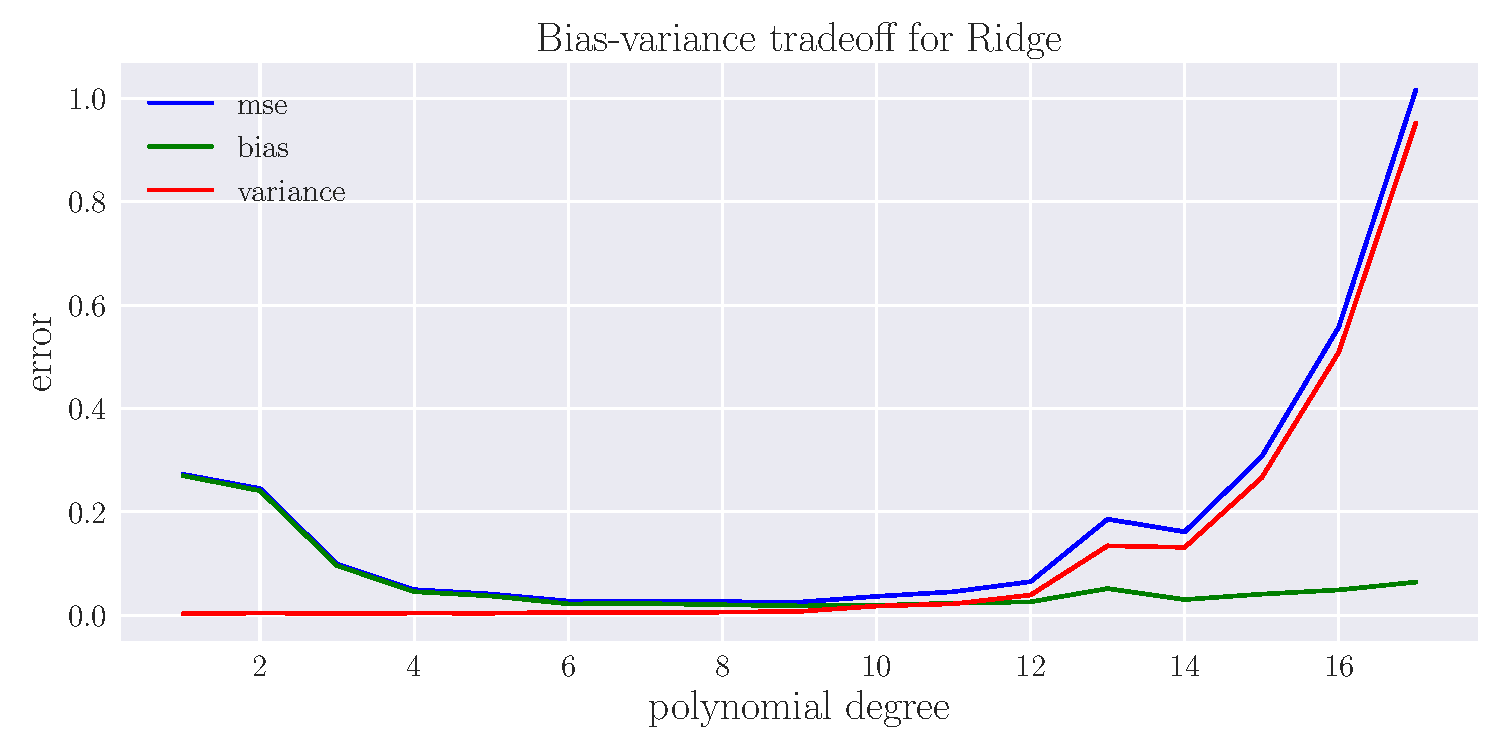
\includegraphics[width=\textwidth]{../output_extra/plots/bias_var_Ridge_c17.pdf}
			\caption{Max degree 17}
			\label{fig:Ridge_a}
		\end{subfigure}
		\hfill
		\begin{subfigure}{0.49\textwidth}
			\centering
			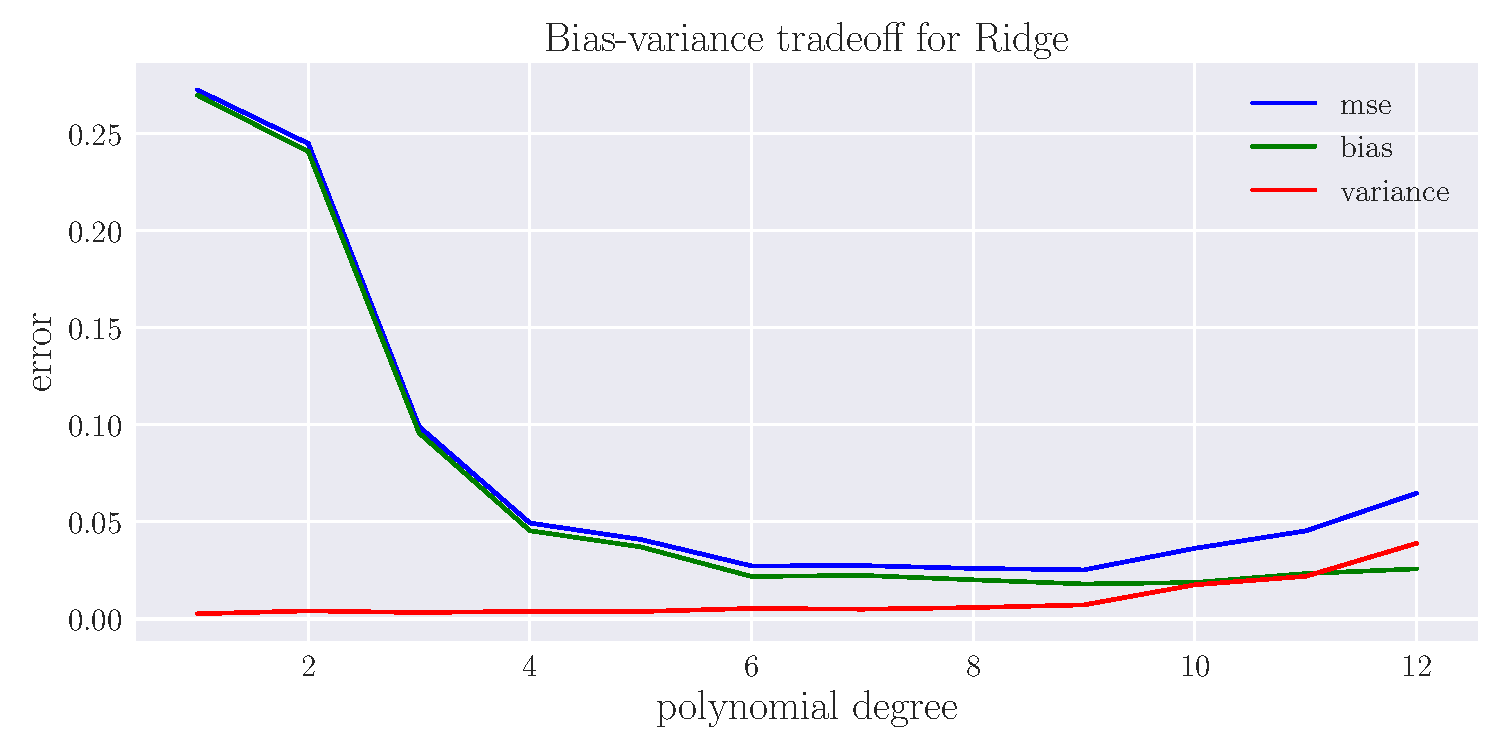
\includegraphics[width=\textwidth]{../output_extra/plots/bias_var_Ridge_c12.pdf}
			\caption{Max degree 12}
			\label{fig:Ridge_b}
		\end{subfigure}
		\caption{Bias-variance tradeoff as a function of polynomial degrees for Ridge, simulated on FrankeFunction. Regularization $\alpha=0.1$.}
		\label{fig:Ridge}
	\end{figure}
	
	Ridge and Lasso regression are alternatives to solve the apparent overfitting problem of OLS. Figure \ref{fig:Ridge} shows the results from Ridge, applying the same polynomial features as for OLS, but now with a regularizaton $\alpha=0.1$. The variance is significantly reduced for same model complexity compared to OLS. The MSE has been reduced to a tractable size even for the highest order polynomials. 
	Adding an $L2$ regularization term better balances the bias and variances. That is, the initial reduction ratio of bias complement the eventual incremental ratio of the variance, resulting in a more symmetric and clear convex  shape of the MSE. \\
	
	\begin{figure}[h]
		\centering
		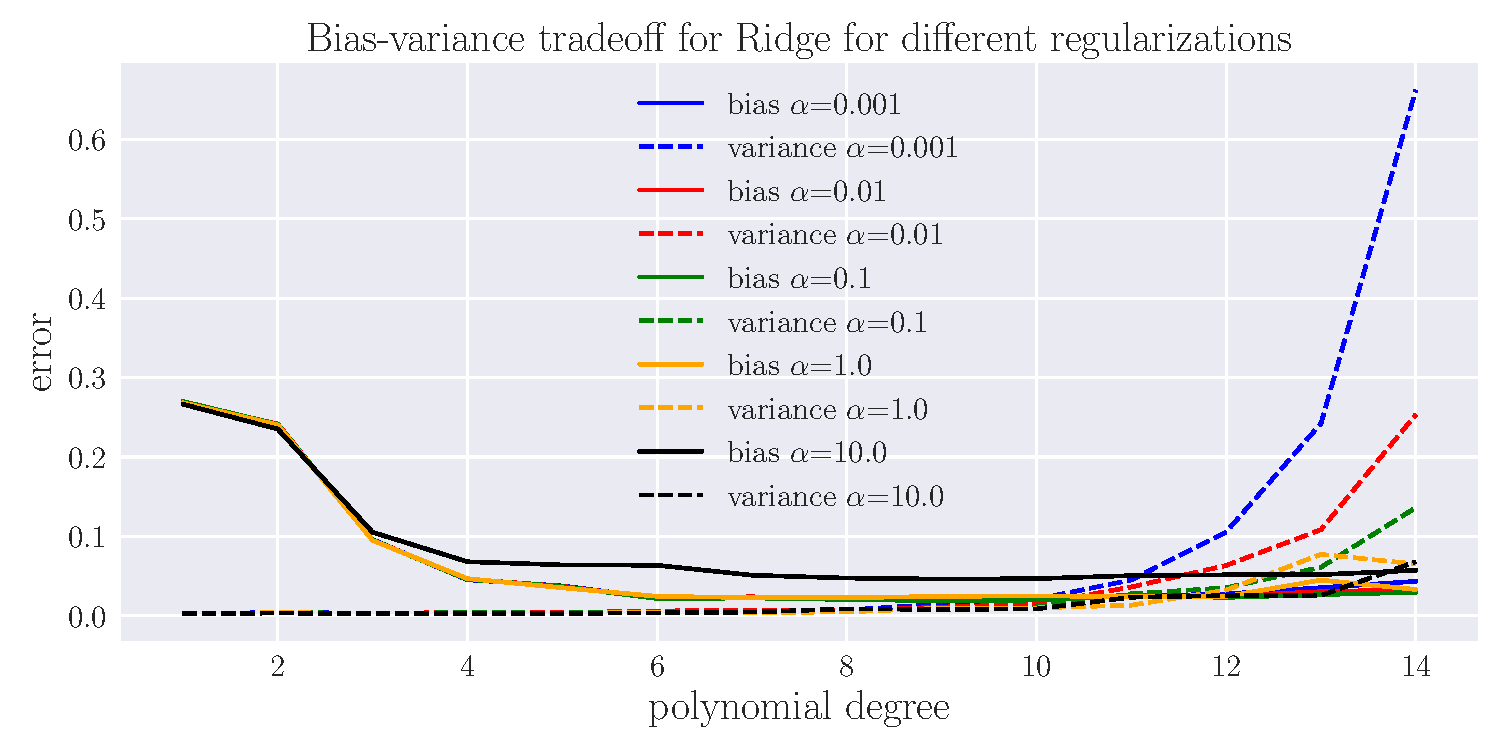
\includegraphics[scale=0.5]{../output_extra/plots/bias_var_Ridge_c14_alpha.pdf}
		\caption{Bias-variance tradeoff for Ridge for different values of regularization $\alpha$.}
		\label{fig:Ridge_alpha}
	\end{figure}
	
	It is of interest to investigate how the bias-variance tradeoff depends on regularization parameter $\alpha$, for Ridge and Lasso. The purpose of the regularization term is to punish large fluctuations of caused by numerous features of the model. Thus, for higher regularization, we expect a simpler and more generalized model. The bias-variance dependency on the $L2$-regularization of Ridge, up to polynomial degree 14, is shown in Figure \ref{fig:Ridge_alpha}. The bias-variance relation is more or less similar for all values of $\alpha$, with an optimal model consistently around polynomial degree 6 and 8. The difference, though, is that increasing $\alpha$ consistently reduces the variance, clearly shown for the highest polynomial degrees. This comes at the expense of a higher bias. Particularly, $\alpha=10$ has the lowest variance for the highest polynomial degree plotted, but clearly attains the largest bias. This indicates that the features of the model have been penalized too severely, at the cost of a too generalized model not able to capture important characteristics of the FrankeFunction. The opposite is the case for the lowest regularization $\alpha=0.001$, where the variance becomes too large for high order polynomials. That is, this Ridge model fits too much of the noise, and is not able to generalize too the more smooth FrankeFunction.
	
	\begin{figure}[h]
		\centering
		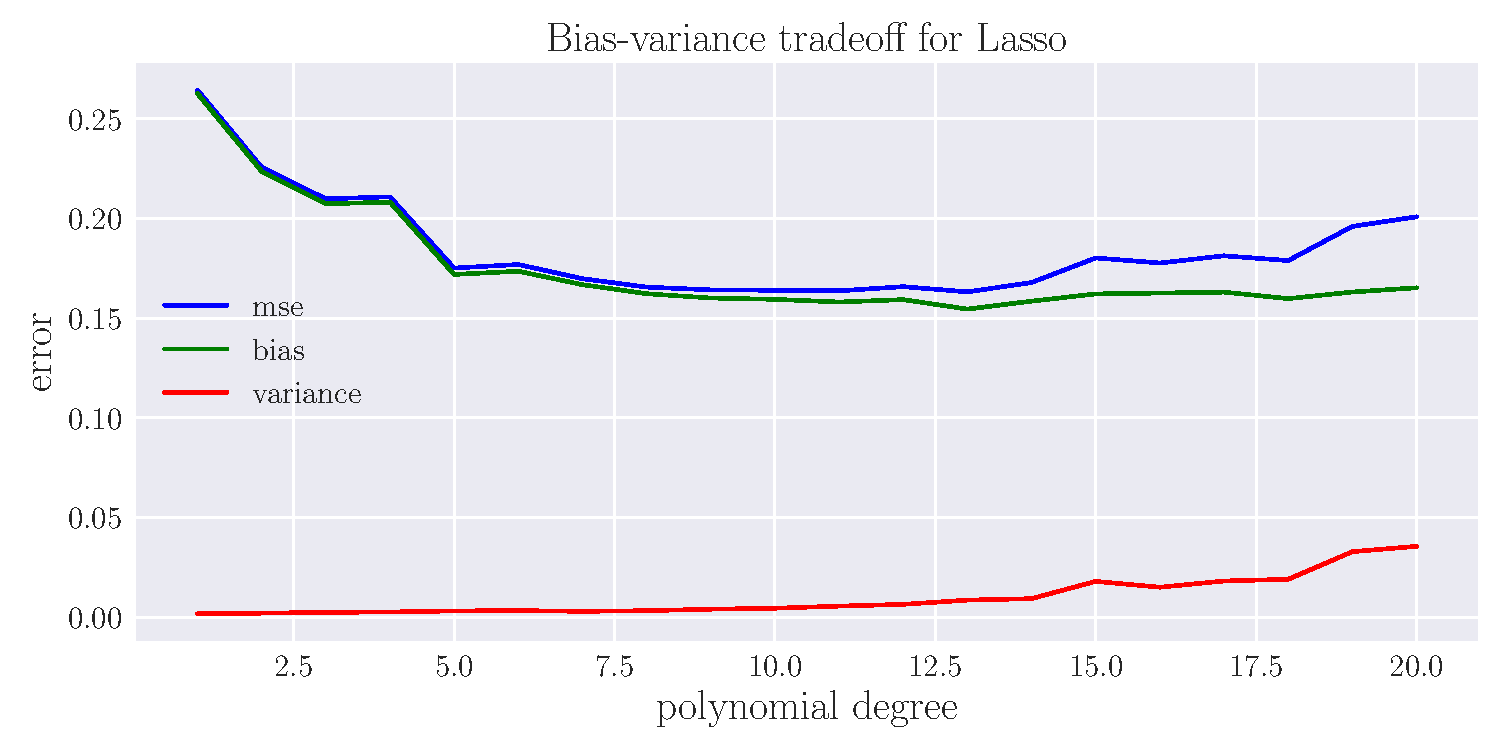
\includegraphics[scale=0.5]{../output_extra/plots/bias_var_Lasso_c20.pdf}
		\caption{Bias-variance tradeoff as a function of polynomial degrees for Lasso, simulated on FrankeFunction. Regularization $\alpha=0.1$. Notice that the simulation is done up to a higher polynomial degree than for OLS and Ridge.}
		\label{fig:Lasso}
	\end{figure}
	
	Simulation of Lasso with a regularization $\alpha=0.1$ is shown in Figure \ref{fig:Lasso}. The variance is signficantly reduced compared to OLS and Ridge. The variance only increases minorly for large model complexity. Most of the MSE clearly consist of bias, which is considerably higher than for OLS and Ridge. Hence $\alpha=0.1$ punishes the features too severely. This has a large impact on the bias-variance tradeoff, as the optimal model for Lasso is achieved for a larger polynomial order, than OLS and Ridge. The model performance clearly suffers from the bias-variance relation for Lasso. 
	
	\begin{figure}[h]
		\centering
		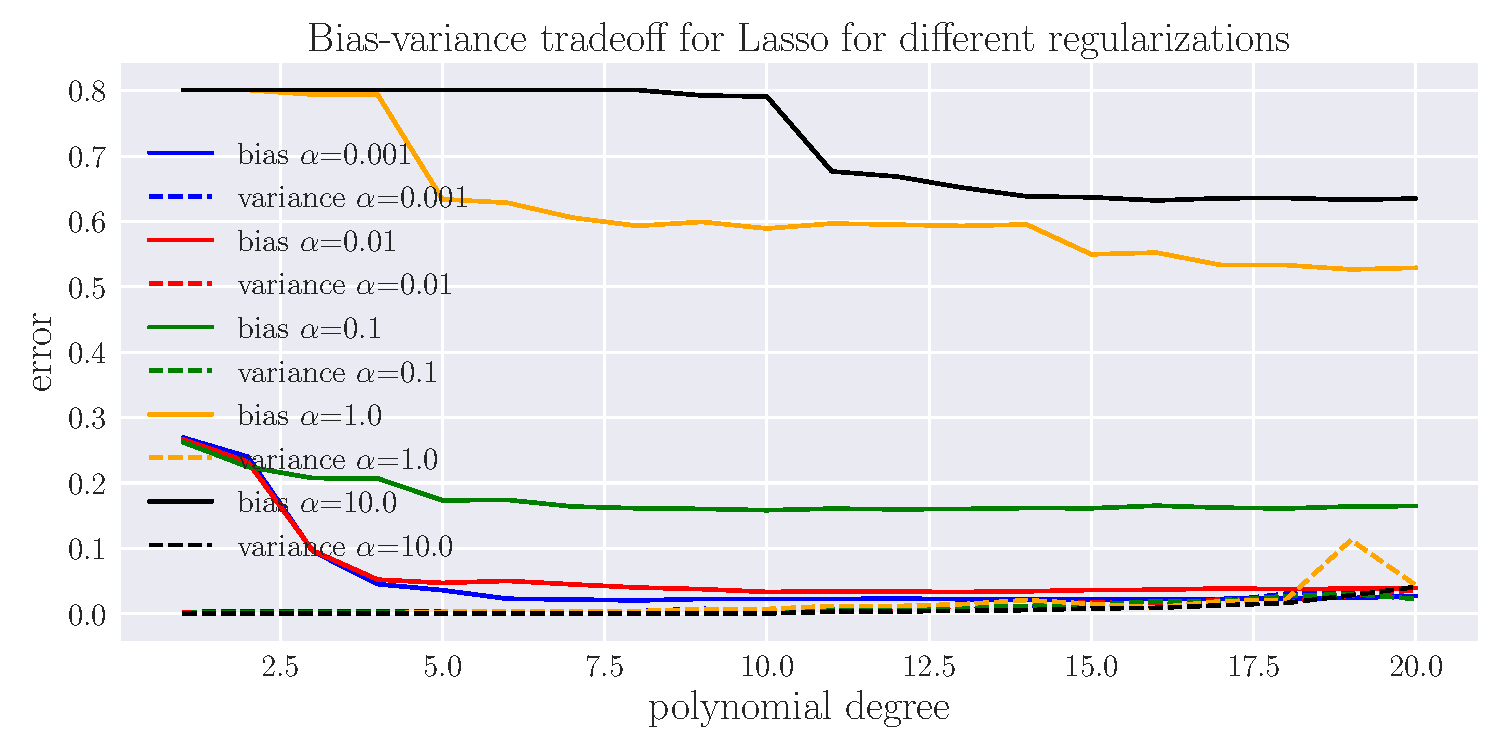
\includegraphics[scale=0.5]{../output_extra/plots/bias_var_Lasso_c20_alpha.pdf}
		\caption{Bias-variance tradeoff for Lasso, for different values of regularization $\alpha$.}
		\label{fig:Lasso_alpha}
	\end{figure}
	
	A comparison of different $\alpha$ is shown in Figure \ref{fig:Lasso_alpha}. The variance remains close to zero for all $\alpha$, even for large polynomial degrees. Bias on the other hand, increases significantly for increased $\alpha$. The implication is a weak bias-variance tradeoff in the sense that, when increasing model complexity, lower bias is not "traded" with higher variance. Instead, the bias remains undesirably large.
	
	\subsubsection*{Neural Network}
	
	\begin{figure}[h]
		\centering
		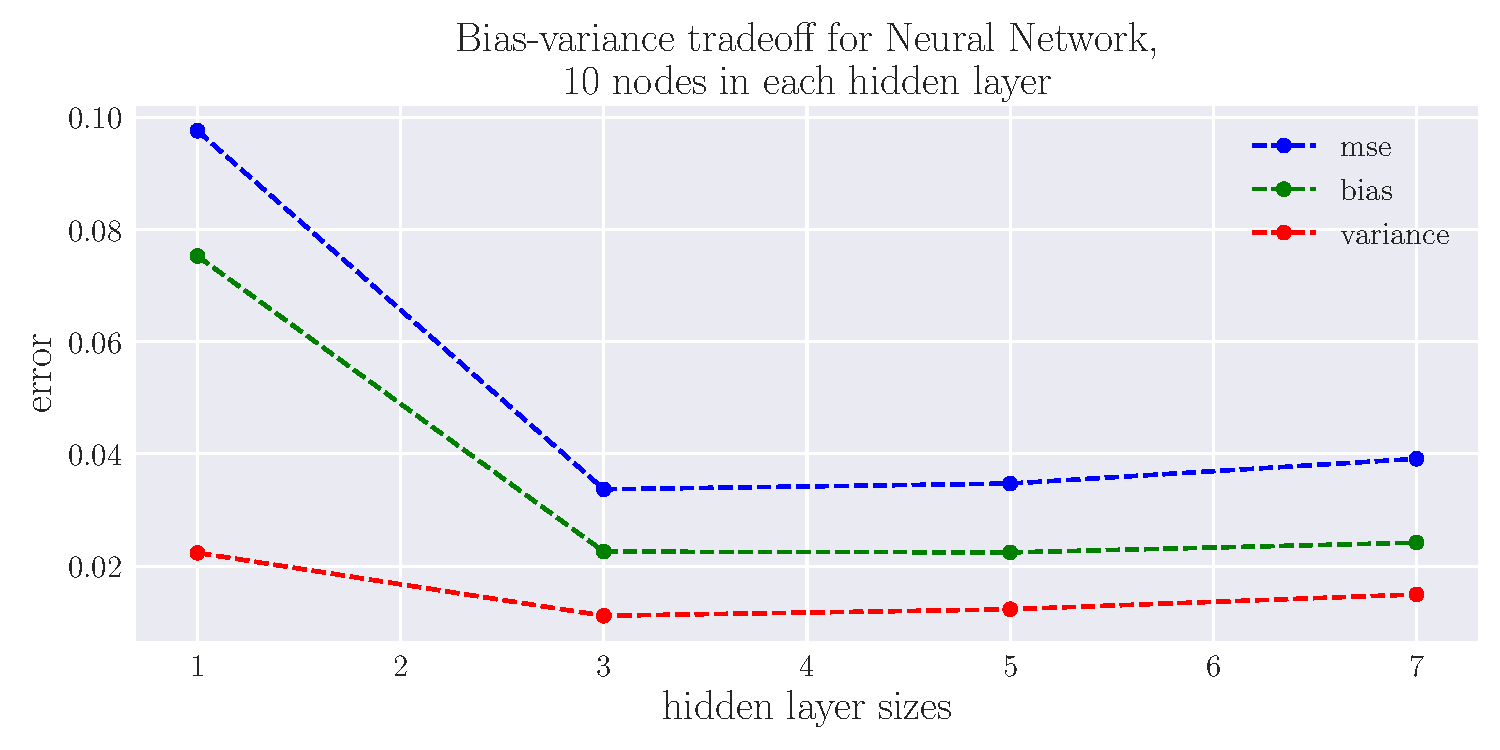
\includegraphics[scale=0.5]{../output_extra/plots/bias_var_NN_layers4_nodes10.pdf}
		\caption{Bias-variance tradeoff for neural network as function of number of hidden layers.}
		\label{fig:NN}
	\end{figure}
	
	Figure \ref{fig:NN} displays the MSE, bias and variance of the neural network class \code{MLPRegressor} trained on the FrankeFunction. The x-axis shows number of hidden layers used, displayed incrementally to go from low complexity to high complexity. Each hidden layer consist of ten nodes. The simulation shows that one hidden layer gives a too general model. By increasing to two hidden layers, the bias decreases significantly. For number of hidden layers beyond two the bias converges to stationarity, whereas the variance increases only slightly. \\

	The bias-variance tradeoff of the neural network reveals an opposite structure to that of OLS. That is, the initial decrease of bias is much larger than the eventual increase of variance. Hence, neural network seems to provide better results for high complexity model with several hidden layers. The bias-variance tradeoff shows similar behaviour to Lasso, in the sense that the bias reaches stationarity while variance increases minorly, yielding an "unsymmetric" tradeoff of bias and variance as a function of model complexity.
	
	\begin{figure}[h]
		\centering
		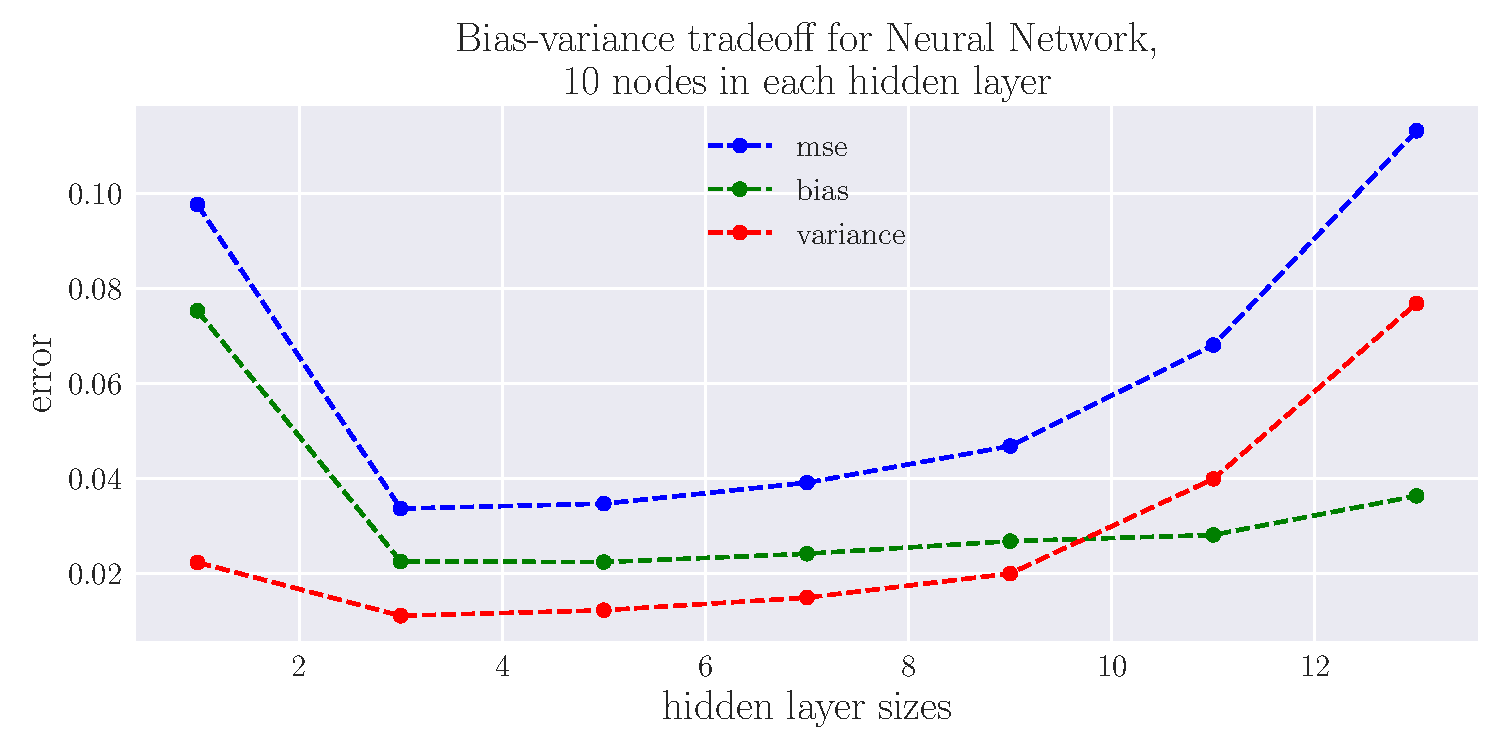
\includegraphics[scale=0.5]{../output_extra/plots/bias_var_NN_layers7_nodes10.pdf}
		\caption{Bias-variance tradeoff for neural network as function of number of hidden layers, now increased to a maximum of 13 hidden layers.}
		\label{fig:NN_complex}
	\end{figure}
	
	A possibility is that maximum number of hidden layers in \ref{fig:NN} is simply not (complex) enough. To unveil this, a plot of even more hidden layers is shown in Figure \ref{fig:NN_complex}. For 13 hidden layers with ten nodes each, the variance becomes large. It implies that we can run a neural network with as many as 10 hidden layers before we really enter the overfitting region. \\
	
	Another distinct feature is that the bias seems to have a slight, almost indiscernable, increase for a model complexity beyond 5 hidden layers. This disproves our statement that the bias reaches stationarity. The overall relationship between bias and variance though, allow us to conclude that the number of hidden layers in a neural network is crucial to obtain an optimal performance and balance between generalization and specification. Because the bias stops decreasing after only three hidden layers, while at the same time variance increases slightly, the best model seems to be three hidden layers.
	
	Using the same number of hidden layers but increasing the number of nodes in each layer, one would expect bias-variance tradeoff to be even more characteristic. That is, overfitting would likely be prominent for even fewer hidden layers, because increasing the number of hidden nodes adds additional complexity. 
	
	
	\subsubsection*{Support Vector Machine}
	
	\begin{figure}[h]
		\centering
		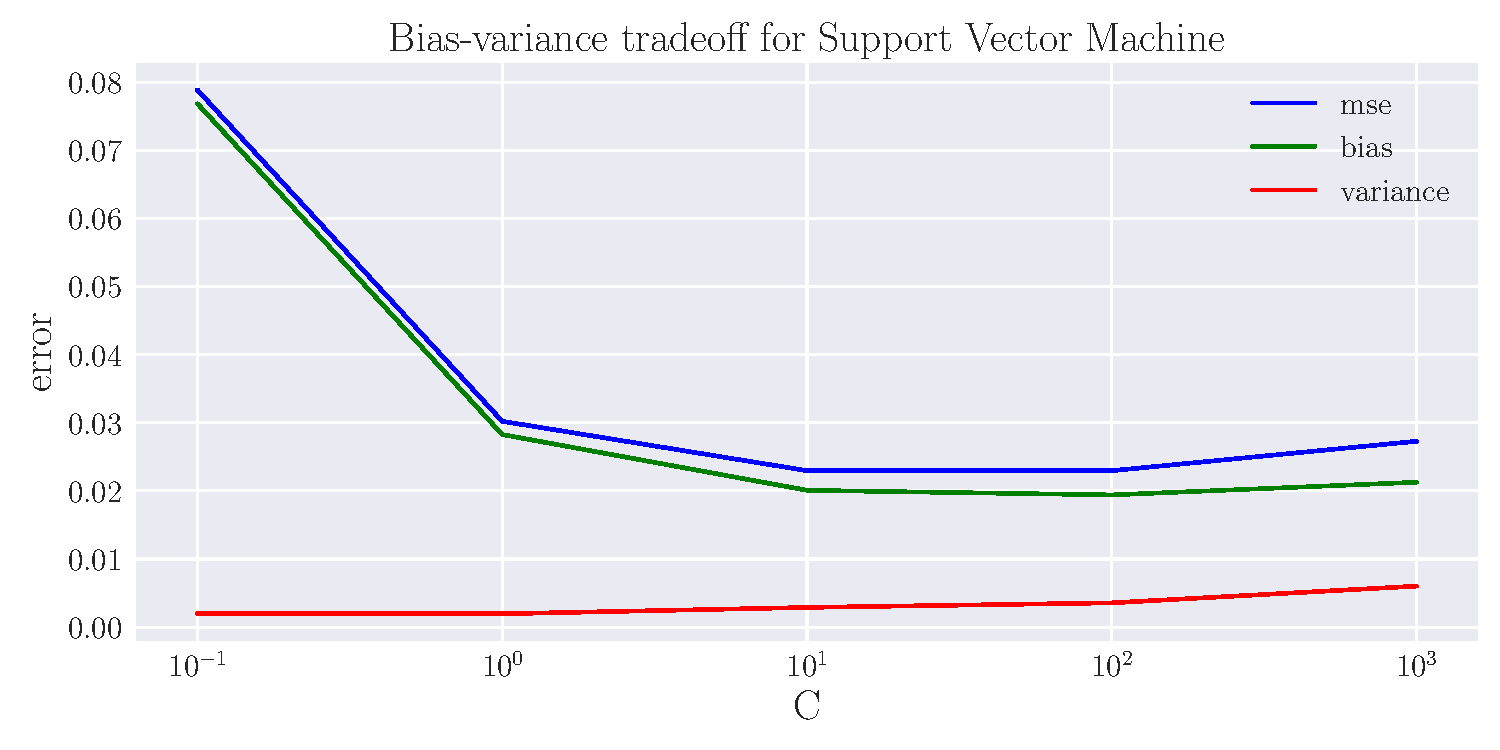
\includegraphics[scale=0.5]{../output_extra/plots/bias_var_SVM_C5.pdf}
		\caption{Bias-variance tradeoff for support vector machine as function of regularization $C$, using $\epsilon=0.2$.}
		\label{fig:SVM}
	\end{figure}
	
	The results from running support vector machine are comparable to linear regression and neural network (Figure \ref{fig:SVM}). For low model complexity, that is a low $C$ parameter, the bias dominates and the model is apparently too simple. For larger $C$ the bias reaches a minimum and actually increases minorly, and so does the variance. Even for $C = 10^4$ the variance remains very low, under 0.01. Still, the slight although almost indiscernible increase is enough to conclude that the best model, yielding an optimal bias-variance tradeoff, is for $C=10$ or $C=100$.
	
	\begin{figure}[h]
		\centering
		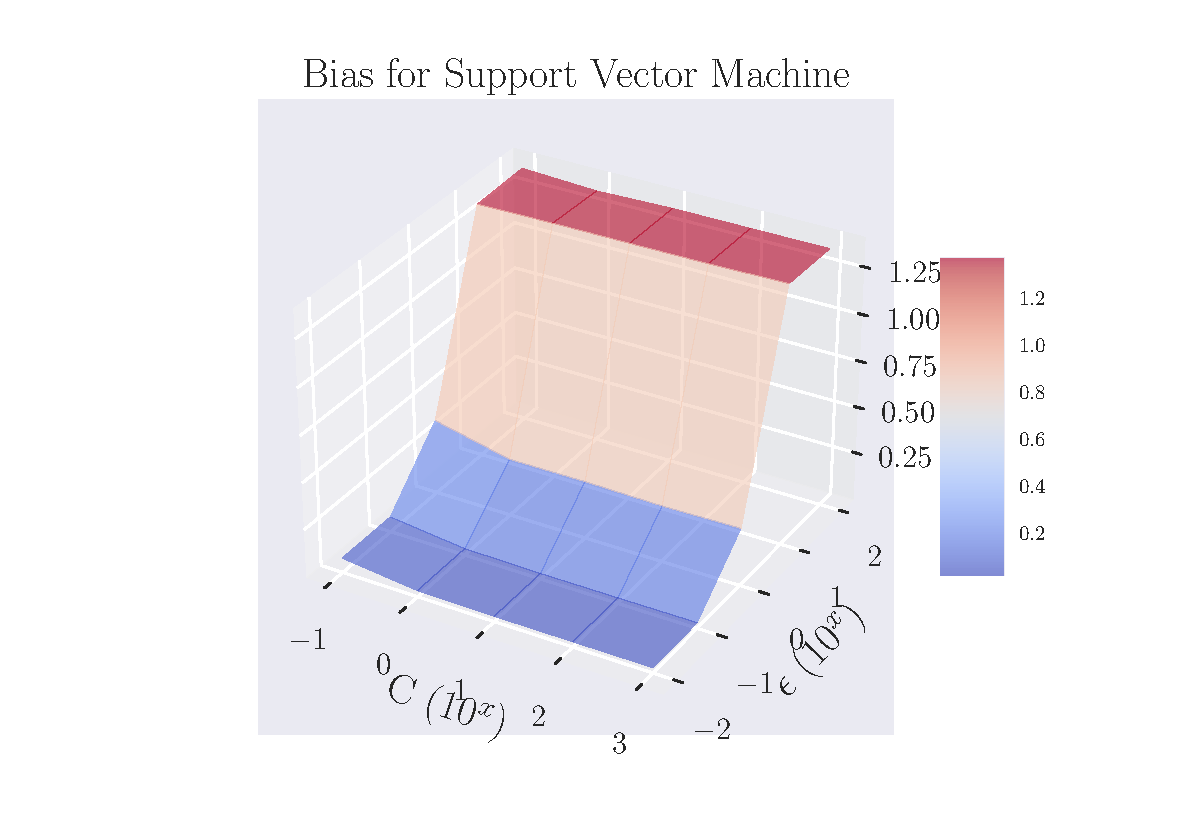
\includegraphics[scale=0.7]{../output_extra/plots/bias_SVM_C5_eps5.pdf}\hfill
		\caption{Bias in the preciction by support vector machine as function of regularization $C$ and residual threshold $\epsilon$. Note the logarithmic scale of horizontal axes.}
		\label{fig:SVM_3d_bias}
	\end{figure}

	\begin{figure}[h]
		\centering
		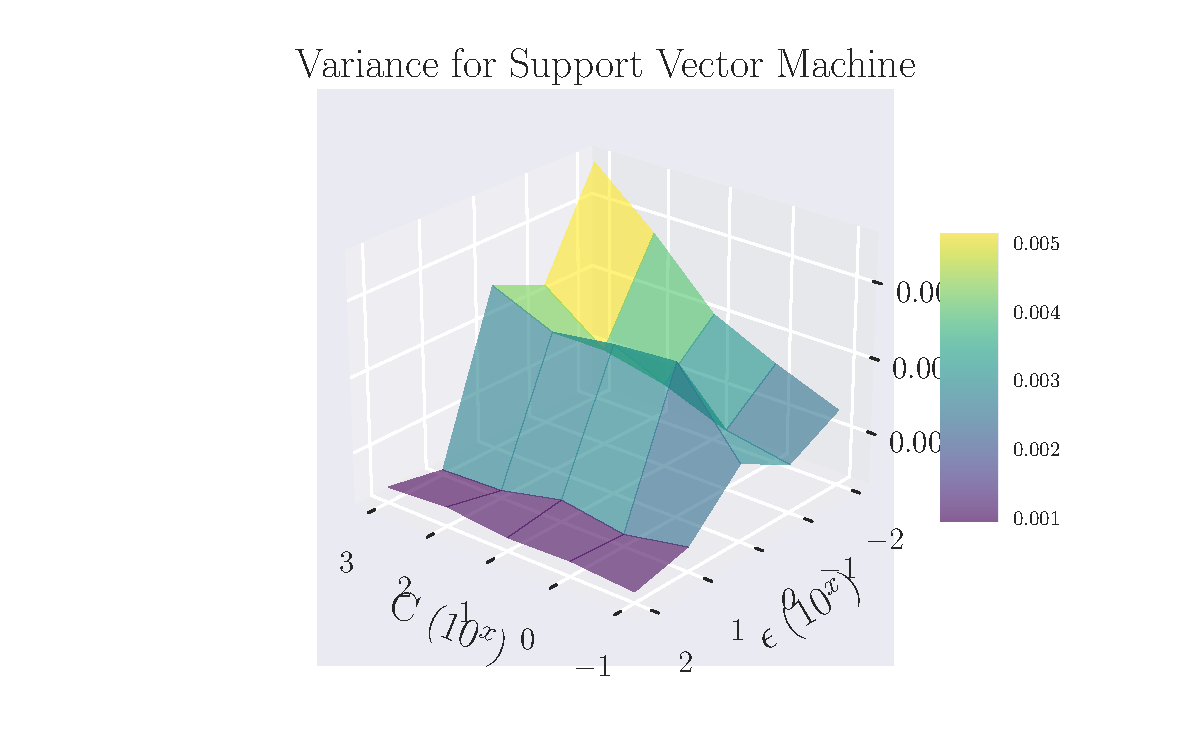
\includegraphics[scale=0.7]{../output_extra/plots/var_SVM_C5_eps5.pdf}
		\caption{Variance in the preciction by support vector machine as function of regularization $C$ and residual threshold $\epsilon$. Note the logarithmic scale of horizontal axes.}
		\label{fig:SVM_3d_var}
	\end{figure}
	
	The most important parameters for optimization of support vector machine are undoubtedly $C$ and $\epsilon$, and we can gain even more insight of the bias-variance tradeoff by including $\epsilon$. Therefore, we decide to bootstrap over both parameters simultaneously. The resulting bias is shown in Figure \ref{fig:SVM_3d_bias} and variance in Figure \ref{fig:SVM_3d_var}. The bias is clearly more sensitive to $\epsilon$ than $C$, at least for the chosen complexities. For the largest $\epsilon$, hardly any support vectors are included in the optimization, which means that the bias reaches a cap. 
	The sensitivity for variance is slightly more distributed across $C$ and $\epsilon$, still dominated by $\epsilon$ though. We observe that the influence of $C$ on the bias-variance tradeoff becomes more prominent for low values of $\epsilon$ (note the gradient of $C$ for low $\epsilon$ in the plot of variance). A suggested explanation is that a larger number of datapoints, namely more support vectors, are affected by the regularization from $C$.
	
	
	\subsection*{Comparison and Conclusion}
	All three methods studied show the same general relationship between bias and variance. Initially the bias is larger and variance is low, and as the model becomes significantly complex the situation is opposite with low bias and high variance. The methods differ in how sensitive the relation is. For example, the variance of OLS shows an exploding tendency for high enough model complexity, whereas for Ridge and neural network (\code{MLPRegressor}) the rate of increase is comparable to the rate of decrease of bias. Lasso stands out by its variance that remain low even for large model complexities (at least those examined). Still, this is the method that yields largest bias, a clear disadvantage in terms of flexibility. Support vector machine is the clear winner when it comes to minimization of error. Its bias-variance tradeoff is reminiscennt of that of Lasso, only that the bias remains consistently low. Conclusively, support vector machine seems to have the least sensitive behaviour of bias and variance, at least when the model complexity is parametrized by $C$, with an overall low error across an array of model complexities. \\
	
	Linear regression benefits from its simple algorithm and impressive runtime, at the same time providing an overall good performance. OLS clearly has a disadvantage by its exploding variance, something that Ridge improves upon. Lasso manages to give low variance across a manifold of model complexities, but suffers from consistently high bias. \\
	
	Neural network takes longer to run than linear regression but gives consistently lower MSE in return. It also has the benefit of obtaining a minimum MSE - and a optimal tradeoff between bias and variance - for a rather low model complexity. Hence, neural network is a powerful and flexible algorithm for training and generalizing quite complex functions. Fitting the FrankeFunction verifies this, as it generally gives low bias and low variance for all model complexities studied. \\
	
	Support vector machine certainly has an advantage by its excellent scores on the test set for a wide range of model complexities. A particular feature is that both low bias and low variance is achieved for high model complexities, at least compared to linear regression and neural network.
	
	Experiments show that using RBF-kernel with $\epsilon=0.2$ the variance does not attain any significant increase for model complexity. This is an important feature of the bias-variance tradeoff characteristic for support vector machines, as opposed to linear regression and neural network, which provides great performance with low bias and low variance for middle to high complexities. This is verified by the simultaneous analysis of $C$ and $\epsilon$ in Figure \ref{fig:SVM_3d_bias} and \ref{fig:SVM_3d_var}, and also from scientific experiments \cite{valentini2004bias}.
	
	The bias-variance tradeoff is not too sensitive, meaning that the gradient of bias and gradient of variance remains low for low and high model complexities, respectively. Though, support vector machine has a significant disadvantage of a large runtime. This is particularly the case using radial basis function kernel combined with a large $C$. Increasing $C$ even further may reveal tendencies of overfitting comparable to linear regression and neural network, but is not investigated due to infeasible computations. From the simultaneous analysis of $C$ and $\epsilon$, we found that the value of $\epsilon$ is very susceptible to the bias. The method is quite sensitive to the number of training samples and linear regression or neural network would probably be a better choice for larger datasets than FrankeFunction \cite{valentini2004bias}.
	
	
	
	
\bibliographystyle{plain}
\bibliography{hastie}
\end{document}